% !TEX root = ../CedricDe Schepper2023_Thesis.tex

\section{Method / Experimental Design}\label{sec:method}
\subsection{Tabu Search}

Tabu search \cite{glover1993} is a meta-heuristic search algorithm based on local search, a heuristic optimisation method that traverses the possible search space by performing local changes to the current solution. Since local search will only accept improving solutions, this traversal can end up being stuck in a local optimum. Tabu search is different from local search by relaxing this rule and also accepting worsening solutions. Additionally, tabu search maintains a memory structure to avoid changes being reversed. The usage of short- to long-term memory is  based on the assumption that optimisation techniques must incorporate memory to qualify as intelligent and that a bad strategic choice is superior to a good random choice\cite{glover1999}. This memory structure is implemented by maintaining a tabu list which contains the x most recent changes performed. A change is thus considered 'tabu' if it is present within the tabu list.
\\\\
Tabu search starts by constructing an initial solution. The solution can be generated randomly or by applying a deterministic approach. During the entire process, the best seen solution to date is maintained. This is necessary due to tabu search allowing worsening changes or so called moves to avoid getting trapped in local minima. After the solution initialisation, the iterative procedure starts searching for a feasible solution. This loop ends when  a specified stopping condition is met. This condition is generally a combination of a solution its objective function scoring below a certain threshold or the procedure reaching a maximum number of iterations.
\\\\
The first step of the main loop is to generate the complete list of possible neighbours of the current solution and ranking them based on the objective function. Subsequently, the best neighbour that is either not tabu or that meets the aspiration criterion is chosen as the next solution. A neighbour is considered tabu if it is present within the tabu list. The aspiration criterion is added to be able to override the tabu requirement. A possible aspiration is to accept solutions that are better than the best seen solution. After choosing the next solution, the best seen solution is updated if the newly generated solution is superior based on the objective function.
\\\\
When the stopping criteria is met, the algorithm ends and the best solution is returned. The full flow of the algorithm can be seen in figure \ref{fig:tabu-chart}.

\begin{figure}[h]
	\centering
	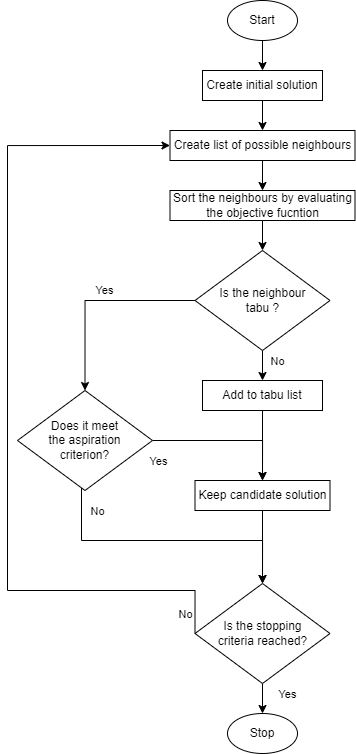
\includegraphics[width=0.5\textwidth]{images/tabu.drawio.png} 
	\caption{Tabu search flow}
	\label{fig:tabu-chart}
\end{figure}

\subsection{Implementation frameworks}

The algorithm implemented to run the experiments is written using Python3.10. The code requires no packages that are not in the Python Standard Library. The profiler cProfiler is used to analyse the performance. It generates a list detailing how long each part of the algorithm runs for and allows to pinpoint and improve bottlenecks.

\subsection{Implementation: version 1}
For this thesis, the initial version or version 1 of the tabu search algorithm to be used in the experiments is based on the algorithm proposed by Alvarez-Valdes et al \cite{alvarez1997}. The algorithm described makes use of a 2-phased approach. During phase 1, the emphasis is on the hard constraints. More specifically, reducing the amount of common students conflicts on the same day is prioritised. Optimally, this initialisation phase would return a solution that is already feasible. The second phase can be considered an optimisation phase, which tries to satisfy the soft constraints as much as possible and thus attempt to distribute the exams evenly.

\subsubsection{Initialisation phase}
The algorithm starts with the initialisation for which the pseudo code is shown in algorithm \ref{alg:phase1}. Firstly, the initial solution must be generated. In the proposed algorithm this is done by randomly assigning all exams to time slots. Generally this will result in several hard constraint violations such as students have more than 1 exam on the same day and room capacity being exceeded. Since Alvarez-Valdes et al consider the room capacity a soft constraint, this is acceptable and will be improved during the iterations. However, in this case, room capacity is seen as a hard constraint that can't be violated at all. In order to circumvent these capacity violations, exams are sorted by student count and only then randomly assigned to time slots with rooms having sufficient capacity. As long as the time slot quantity and room capacity is sufficient, this will result in a solution with no room capacity violations. Another added complexity is the presence of different room types which was not the case for Alvarez-Valdes et al. In order to satisfy constraint 2, only rooms with a suitable type are considered when assigning exams to time slots.

\begin{algorithm}
 Generate an initial solution s in the space of solutions X\;
 $s^* = s$ (with $s^*$ the best solution seen so far)\;
 $k = 0$ (with k the number of iterations)\;
 \While{k < maximum number of iterations and $f(s^*) \neq 0$}{
  $k = k + 1$\;
  \tcc{perform single moves of one exam to another time slot}
  Generate set of solutions $V^* \subseteq N(s, k)$\ (set of neighbours of s)\;
  Sort $V^*$ by ascending $f(s')$ and select the best $s'$\;
   \ForEach{solution $s'$ in $V^*$}{
    \If{not $tabu(s')$ or $f(s') < f(s^*)$ (aspiration criterion)}{
        $s = s'$\;
        \textbf{break}\;
    }
   }
   \If{$f(s') < f(s^*)$}{
   $s^* = s'$\;
   }
 }
 \KwRet{$s^*$}

\caption{Initialisation phase}
\label{alg:phase1}
\end{algorithm}

After generating the initial solution, the iterative procedure starts by generating the set of neighbours of the current solutions. We consider a solution $s' \in X$ a neighbour of $s \in X$, whenever we can move an exam to a time slot in a different period. Evaluating the entire search space would be too time consuming. Instead, we first sort all periods by its contribution to the objective function. From the most conflictive period, we select the most conflictive time slot. Finally, we calculate all available time slots that we can swap with. In order to swap two time slots, the two affected exams (or sole affected exam when swapping to a time slot with no scheduled exam) must be able to be scheduled in the new time slots keeping the room type and capacity into account. This will ensure that no additional constraint 2 and 3 violations are introduced.

For each possible move, the objective score is calculated in order to rank all neighbours. The objective function for a solution $s$ can be defined as

\begin{equation}
    f(s) = \sum_{i=1}^{N} ( \sum_{j,k \in E_i}^{}p x_{jk})
\end{equation}
with $N$ the amount of periods, $E_i$ the set of exams scheduled to period $i$, $x_{jk}$ the number of common students between exams $j$ and $k$,
and $p$ the weight of conflicts.

After sorting all found neighbours by objective function, the best solution, that is not tabu or for which the aspiration criterion applies, is chosen. The aspiration criterion accepts solutions that are tabu as long as they are superior to $s^*$ (the best solution seen so far) If no moves are possible, we select the next most conflictive time slot until a suitable move has been found. When choosing the new solution, the tabu list is updated with the new tabu move consisting of the exam and period involved. Whenever the tabu list exceeds its maximum size, the oldest move is deleted, in order to allow that move again in future iterations.

This phase runs until a solution without conflicts has been found or the maximum number of iterations has been reached. For the latter case, the schedule will have conflicting exams during the same period with common students.

\subsubsection{Optimisation phase}

After the initialisation phase, we start the optimisation of the solution. Here the focus is including the soft constraints in the objective function to generate a solution that is the most optimal. The foundation of this phase is similar compared to the first phase with some distinct features. The overall flow can be seen in the pseudo code described in algorithm \ref{alg:phase2}.

\begin{algorithm}
\KwData{Solution s (the result of the initialisation phase)}
 $s^* = s$ (with $s^*$ the best solution seen so far)\;
 $k = 0$ (with k the number of iterations)\;
 \While{k < maximum number of iterations and $f(s^*) \neq 0$}{
  $k = k + 1$\;
  \uIf{$k\ \mathbf{mod}\ 3 \neq 0$}{
  \tcc{perform single moves of one exam to another time slot}
    Generate set of solutions $V^* \subseteq N(s, k)$\ (set of neighbours of s after single move)\;
  Sort $V^*$ by ascending $f(s')$ and select the best $s'$\;
   \ForEach{solution $s'$ in $V^*$}{
    \If{not $tabu(s')$ or $f(s') < f(s^*)$ (aspiration criterion)}{
        $s = s'$\;
        \textbf{break}\;
    }
   }
  }
  \Else{
    \tcc{swap entire period}
    Generate set of solutions $V^* \subseteq N(s, k)$\ (set of neighbours of s after swapping periods)\;
    Sort $V^*$ by ascending $f(s')$ and select the best $s'$\;
    $s = s'$\;
  }
  
   \If{$f(s') < f(s^*)$}{
   $s^* = s'$\;
   }
 }
 \KwRet{$s^*$}

\caption{Optimisation phase}
\label{alg:phase2}
\end{algorithm}


Firstly, the objective function is updated to take the distribution of exams into account. The objective of a solution is now defined as

\begin{equation}
    f(s) = \sum_{i=1}^{N} \sum_{j=1}^{N}(p_{|i-j|} \sum_{k \in E_i}^{}\sum_{l \in E_j}^{} x_{kl})
\end{equation}
with $N$ the amount of periods, $E_i$ the set of exams scheduled to period $i$, $x_{kl}$ the number of common students between exams $k$ and $l$, and $p_{|i-j|}$ the penalty for two exams scheduled at a distance of $|i-j|$ periods or days. While the objective function in the first phase only used the common students between exams during the same period, the new objective function will take all combination into account. By having a large penalty $p_0$ for exams scheduled on the same day, the hard constraint of having no exams on the same day for a student is still being prioritised. Additionally, placing exams at a further distance will now be preferred since the penalty $p_{x+1}$ will be smaller than the penalty $p_x$.

Secondly, two options are now available when generating the set of neighbours of the solution. The first option is a copy of the process in the initialisation phase where the set of neighbours of the solution is generated by performing single moves. Then the best solution that is either not tabu or that meets the aspiration criterion will be used. While this option might introduce constraint violations, the high $p_0$ will discourage and depending on the values used prevent this. This method will be alternated with a period permutation. Instead of moving a single exam, two entire periods will be swapped. Since the exams in the periods are not updated, this swap can not introduce any hard constraint violations. By moving entire periods, the objective function can change significantly in a single move. However, the amount of available moves is much lower and can be defined as
\begin{equation}
\begin{split}
   \text{\# possible moves}  & = \binom{N}{2}   \\
   & = \frac{N!}{2!(N-2)!}
\end{split}
\end{equation}

\subsection{Implementation: version 2}

After running experiments using version 1, some run time and result characteristics were observed. Version 2 diverts even more from the original algorithm in order to avoid these occurrences. Firstly, the objective function originally defined in the initialisation phase as   
\begin{equation}
    f(s) = \sum_{i=1}^{N} ( \sum_{j,k \in E_i}^{}p x_{jk})
\end{equation}
has an unwanted characteristic: it does not punish students with several exams on the same day extra. For exam schedules without a conflict free solution, this often results in students, who are enrolled in smaller exams, having a large number of exams on the same day. In order to avoid this behaviour, the objective function is updated to
\begin{equation}
    f(s) = \sum_{i=1}^{N} ( \sum_{s \in S(E_i)}^{}p^{c_{si} - 1})
\end{equation}
with $N$ the amount of periods, $E_i$ the set of exams scheduled to period $i$, $S(E_i)$ the set of students with more than 1 exam during $E_i$, $c_{si}$ the number of exams student $s$ has on period $i$, and $p$ the weight of conflicts. By placing $c_{si}$ in the exponent, having multiple exams on the same day is punished severely. 

Secondly, the way a tabu move is defined was changed. Originally, when moving an exam to a different period, the combination of the exam and period was used to define the tabu move. This resulted often resulted in the scenario that the same exam was continuously being moved. since this generally was one of the largest exams, it always has a large impact on the objective function and kept being determined as the most conflictive time slot. This behaviour can be avoided by having the exam as the sole identifier of the tabu move. By doing this, a single exam will not be moved as frequently.

\subsection{Implementation: version 3}

Version 1 and 2 both reduce the search space by only looking at the most conflictive time slot of the most conflictive period in order to determine the possible moves. Different time slots are only looked at when no moves are possible. This version steps away from that principle and continues evaluating the next most conflictive time slots their possible moves until a specified amount of possible moves have been found. Only then it selects the move generating the best next solution.



